\chapter{Algebraic Structure}


\begin{summary}
	Let $ A:V\to W $ be a linear map between vector spaces. Then the pre-image of any linearly independent set contains a linearly independent set. Let $ \set{w_n} $ be a linearly independent set of vectors in $ W $. Let $ v_n = \inv{A}(w_n) $, i.e. \textbf{one} of the pre-images of $ w_n $ (if $ A $ is not injective, then $ w_n $ can have multiple pre-images. But we choose just one pre-image. Any of them will work). Then let $ \sum_n \beta_n v_n = 0 $. Using the fact that $ v_n = \inv{A}(w_n) $, one can write
	\[ 0 = A(\sum_n \beta_n v_n) = \sum_n \beta_n A(\inv{A}(v_n)) = \sum_n \beta_n w_n,  \]
	which implies $ \beta_n = 0 $ for all $ n $. So $ \set{v_n} $ is linearly independent.
	
	But note that the image of a linearly independent set is not necessarily a linearly independent set. Because a linear map can collapse some of the vectors to the origin, and the resulting collection will not be a linearly independent set of vectors. 
\end{summary}

\begin{summary}
	Even in infinite dimensional vector spaces, an infinite sum of the form $ \sum_{n=1}^{\infty} \alpha_n v_n $ for $ \alpha_n \in F $ and $ v_n\in V $ for all $ n $, is  meaningless, and one needs a topological structure on the space to make sense of such infinite sums.
\end{summary}


\begin{summary}[Causality and subspaces]
	Consider the space of functions defined on the real line (no regularity condition is necessary). Denote this space with $ X $. Let $ A:X\to X $ be a linear map between these two space, and let $ L_T $ denote the subspace that $ x\in L_T $ iff $ x(t) = 0 $ for all $ t\leq T $. $ L $ is a causal map iff $ L_T $ is invariant under $ A $, that is $ A(L_T) \subset L_T $.
	
	\begin{proof}
		Assume $ A $ is causal map and we want to show that $ L_T $ is invariant. Let $ x\in L_T $. So $ x(t) = 0 $ for all $ t\leq T $. The origin $ x_0 \in L_T $ also satisfies $ x_0(t)=0 $ for all $ t\leq T $. From causality of $ A $ we need to have $ [Ax](t) = [Ax_0](t) $ for all $ t\leq T $. Since $ A $ is linear it sends the origin to the origin, i.e. $ A(x_0) =0 $. This implies $ [Ax](t) =0 $ for all $ t\leq T $. So $ Ax \in L_T $. So $ L_T $ is invariant under $ L $.
		
		Now assume $ L_T $ is invariant under $ A $ and we want to show that $ A $ is causal. Let $ x,y\in X $ with $ x(t) = y(t) $ for all $ t\leq T $. Then $ (x-y)(t) = 0 $ for all $ t\leq T $, this $ x-y\in L_T $. So is $ A(x-y) = Ax - Ay $. So $ (Ax-Ay)(t) = 0 $ for all $ t\leq T $. So $ [Ax](t) = [Ay](t) $ for all $ t\leq T $. So $ A $ is causal.
	\end{proof}
\end{summary}
\begin{summary}
	Not that $ \cup_\alpha B_\alpha $ can be a linear subspace and in the \autoref{prob:intersectionOfSubspaces} we did not rule out the possibility of $ \cup_\alpha B_\alpha $ to be a linear subspace. For instance, consider the space of all functions defined on the real line $ X $, and let $ X_T $ denote the subspace of functions that vanish to the left of $ T\in\R $, i.e. $ x(t) = 0 $ for all $ t\leq T $. In this case $ \cup_T X_T $ is the space of all functions that vanishes to the left of some finite time. This is a subspace of $ X $.
\end{summary}


\begin{summary}
	It is well know that the set of all linear transformations from a linear space to another linear space is itself a linear space. However, there is even more! Let $ X $ be an arbitrary nonempty set and let $ Y $  be a linear space. Then $ \mathcal{F} $, the set of all mappings of $ X $ into $ Y $, is a linear space (with the addition of mappings and scalar multiplies of mappings are defined as in Example 2 Section 2. 
\end{summary}


\begin{summary}
	A linear transformation is one-to-one (injective) if its kernel only contains the origin.
	\begin{proof}
		Let $ L $ be injective, and let $ a\in \ker L $. Then $ La = 0 $, and from linearity of $ L $ we have $ L0 = 0 $. From injectivity of $ L $ we must have $ a =0  $.
		
		Let $ \ker L = \set{0} $. Let $ x,y\in V $ such that $ f(x) = f(y) $. Then from linearity of $ f $ we can write $ f(x-y) = 0 $. Since the kernel only contains the origin we will have $ x-y= 0 $, so $ x= y $.
	\end{proof}
\end{summary}

\begin{summary}
	The inverse of a linear transformation, if exists, is linear. 
	\begin{proof}
		Let $ L:V\to V $ be a linear transformation that its inverse exists denoted by $ \inv{L} $. Let $ y_1,y_2 \in V $. Then exists $ x_1,x_2\in V $ such that $ y_1 = Lx_1 $ and $ y_2 = Lx_2 $. Consider
		\begin{align*}
			\inv{L}(\alpha y_1 + y_2) = \inv{L}(\alpha Lx_1+ Lx_2) = \inv{L}(L(\alpha x_1+x_2)) = \alpha x_1 + x_2  = \alpha\inv{L}(y_1) + \inv{L}(y_2).
		\end{align*}
		So $ \inv{L} $ is linear when exists.
	\end{proof}
\end{summary}


\begin{summary}
	Let $ X = l_2(-\infty,\infty) $ and $ Z $ be the linear space made up of all complex-valued functions $ f(z) $ defined on the unit circle of the complex plane such that
	\[ \frac{1}{2\pi i} \int_C \abs{f(z)}^2 dz/z <\infty. \]
	The usual assumption is made that if $ f_1(z) $ and $ f_2(z) $ differ only on a set of measure zero, then $ f_1 $ and $ f_2 $ are considered to be the same function. These two spaces are isomorphic as linear spaces with
	\[ (\cdots,\xi_{-1},\xi_0, \xi_1,\cdots) \mapsto f(z) \]
	with
	\[ f(z) = \sum_{n=-\infty}^{\infty}\xi_n z^{-n}. \]
	This is the two-sided z transform.
 \end{summary}
 \begin{remark}
 	In the example above, using appropriate change of variable, and utilizing the fact that functions in $ Z $ are defined on the unit circle we can write
 	\[ \frac{1}{2\pi i}\int_C \abs{f(z)}^2 dz/z = \frac{1}{2\pi i}\int_{0}^{2\pi}\abs{f(e^{i\theta})}^2 d\theta. \]
 	In the second form, the connection to the Fourier transform is more clear.
 \end{remark}
 \begin{remark}
 	In the example above, the subspace $ L \subset X$ where $ x\in L $ if $ x_i=0 $ for all $ i<0 $ maps to the Hardy space $ H^2 $ via the constructed isomorphism. Hardy space is the space of all that are restriction of harmonic functions to the unit sphere.
 \end{remark}
 
 
 \begin{summary}[Some definitions]
 	There are some important nuances in some definitions in linear algebra. We will highlight those definitions here.
 	\begin{definition}[Linear Combination]
 		Let $ V $ be a vector space, and $ A\subset V $. Then $ x\in V $ is said to be a linear combination of elements in $ A $ if there is a \textbf{finite} sum such that
 		\[ x = \sum_{i=1}^{n}\alpha_i v_i, \quad v_i \in A \text{ for all $ i $}. \]
 		Accordingly, $ \vspan{A} $ is defined to be the set of all \textbf{finite} linear combinations of $ A $.
 	\end{definition}
 	\begin{remark}
 		Regardless of the nature of the linear space (finite or infinite dimensional), a linear combination is always a finite sum.
 	\end{remark}
 	\begin{proposition}
 		For any collection of vectors $ A \subset V $, $ \vspan{A} $ is \textbf{the smallest subspace} of $ V $ that \textbf{contains} $ A $.
 	\end{proposition}
 	
 	\begin{proposition}[Linear Independence]
 		Let $ A\subset V $ be a collection of vectors. Then the followings are equivalent.
 		\begin{enumerate}[(a)]
 			\item $ A $ is a linearly independent set of vectors.
 			\item For every $ x\in A $ we have $ x\notin\vspan{A\backslash\set{x}} $. That is $ x $ is not a linear combination of the points in $ A\backslash\set{x} $.
 			\item For every \textbf{finite} sub-collection $ \set{v_1,\cdots,v_n} \subset A $ we have
 			\[ \sum_{i=1}^{n}\alpha_i v_i = 0 \quad \implies \quad v_i = 0 \quad \forall i=1,\cdots,n. \]
 			\item For $ v\neq 0 \in \vspan{A} $ there exists one and only one finite subset of $ A $, say $ \set{v_i}_{i=1}^n $ and a unique $ n $-tuple of non-zero elements such that
 			\[ v = \sum_{i=1}^{n} \alpha_i v_i.  \]
 			
 			\item $ A $ a linearly independent set of vectors if and only if there exists no proper subset $ A_0 \subset A $ such that $ \vspan{A_0} = \vspan{A} $. I.e. for all $ B \in 2^A $ one has $ \vspan{B} \subseteq \vspan{A} $.
 		\end{enumerate}
 	\end{proposition}
 	\begin{remark}
 		Note that in item (d) above we have excluded the origin, and also forced the $ n $-tuple to have non-zero elements. Because $  0 = 0 v_1 + 0v_2 = 0v_3 + 0v_4 $, etc assuming $ v_1,v_2,v_3,v_4\in A $. Furthermore, let $ v \in A $, that trivially $ v\in \vspan{A} $. Then one can write $ v = 1v $, $ v=1v+0v_1 $, etc. I.e. one can add more vectors from $ A $ with zero coefficients.
 	\end{remark}
 \end{summary}
 
 
 \begin{summary}
 	In Example 5, page 179, we discuss a very important example about the subspace $ A_x \subseteq l_2(-\infty,\infty) $ and its connection to $ Z $, the set of all complex valued functions defined on $ \mathbb{T} $ such that 
 	\[ \int_C \abs{f(z)}^2 dz/z = \int_{0}^{2\pi} \abs{f(e^{i\theta})}^2d\theta < \infty. \]
 	$ Z $ and $ l_2(-\infty,\infty) $ are isomorphic via $ \phi $ given as:
 	\[ (\cdots,\xi_{-1}, \xi_{0},\xi_{1},\cdots) \mapsto \sum_{n=-\infty}^{+\infty} \xi_n z^{-n}. \]
 	It turns out
 	\[ \phi[S_r^n x](t) = t^{-n} \phi[x](t), \]
 	i.e. shifting the sequence $ x $ to the right by $ n $-positions, is the same as multiplying $ [\phi x](t) $ be the monomial $ t^{-n} $. So $ A_x = \set{\sum_{n=M}^{N}\alpha_n S_r^n x} $ is the same as $ L\subset Z $ given by
 	\[ L = \set{g(t)\cdot [\phi x](t): g(t)\text{ is a Laurent polynomial}}. \]
 	A Laurent polynomial is a polynomial in variables $ z $ and $ 1/z $.
 	
 	\begin{remark}
 		 The importance of the monomial like $ f(z) = z^n $ becomes more evident when one restricts $ f $ to the unit-circle in the complex domain, i.e. $ \mathbb{T} = \set{\abs{z}=1} $. Because
 		 \[ f\big|_{\mathbb{T}}(z) = f(e^{i\theta}), \quad \text{where }z=e^{i\theta}. \]
 		 Thus restricting $ f(z)=z $ to $ \mathbb{T} $ we will get
 		 \[ f(e^{i\theta}) = e^{in\theta} = cos(n\theta) + i\sin(n\theta). \]
 	\end{remark}

 \end{summary}
 
 \begin{summary}[More intuition about the basis]
 	We know that if $ A $ is linearly independent, then every non-zero vector in $ \vspan{A} $ has a unique linear combination of the vectors in $ A $. With this characterization of linear independence, and appropriate definition of spanning, we can have the following proposition.
 	\begin{proposition}
 		$ A\subset X $ is a basis if and only if every non-zero vector has a unique linear combination of vectors in $ A $.
 	\end{proposition}
 \end{summary}
 
 \begin{summary}
 	Let $ X = \ell(\R) $ be the space of real sequences. Then one might tend to think that the set $ A = \set{e_1, e_2,\cdots} $ where $ e_i[j]=\delta_{ij} $, i.e. the $ i^\text{th} $ position of $ e_i $  is non-zero (equal to one). But this set is not a basis. Because one can not write the sequence with infinite support as a finite linear combination of elements in this collection. In fact $ \vspan{A} $ is a proper subspace of $ X $ consisting of all sequences with finite support.
 \end{summary}
 
 \begin{summary}
 	Some useful facts
 	\begin{enumerate}[(a)]
 		\item Cardinality of the Hamel basis of a vector space is the dimension of the space.
 		\item Two Hamel bases for a fixed space have the same Cardinal numbers.
 		\item Two vector spaces are isomorphic if and only if the have the same dimension.
 	\end{enumerate}
 	\begin{proof}
 		\begin{enumerate}[(a)]
 			\item It is a definition!
 			\item See Appendix B in the text book
 			\item Let $ B_1 $ be a basis for $ V_1 $ that is isomorphic to $ V_2 $ via $ \phi $. Then $ \phi(B_1) $ is a basis for $ V_2 $ and since $ \phi $ is a bijection, then $ B_1 $ and $ \phi(B_1) $ both has the same cardinality. For the converse, assume $ B_1 $ and $ B_2 $ has the same cardinality so there is a bijection between these two sets. Let $ \phi $ be a linear map that maps the bases to bases according to the bijection. This is a linear map and is a bijection by construction. So $ V_1 $ and $ V_2 $ are isomorphic.
 		\end{enumerate}
 	\end{proof}
 \end{summary}
 

 
 
 \begin{summary}[Facts about subspaces]
 	Consider the following two propositions.
 	\begin{proposition}
 		Let $ V $ be a linear space and $ A\subset V $ be a set of vectors. Then $ a \implies b $ and $ b,c $ are equivalent.
 		\begin{enumerate}[(a)]
 			\item $ \vspan{A} $ is the set of all linear combinations of vectors in $ A $.
 			\item $ \vspan{A} $ is the smallest subspace containing $ A $.
 			\item $ \vspan{A} $ is the intersection of all subspaces containing $ A $.
 		\end{enumerate}
 		\begin{proof}
 			The equivalence between (b), and (c) is merely the definition of intersection. Now we want to establish $ a\implies b $. The fact that $ \vspan{A} $ contain $ A $ and $ \vspan{A} $ are easy. We will show that $ \vspan{A} $ is the smallest such space. So we prove that $ \forall W \subset V $ a linear subspace, if $ A \subset W $ then $ \vspan{A} \subset W $. Let $ W $ be any subspace that contains $ A $, and let $ x \in \vspan{A} $. Then $ x $ is a linear combination of the points in $ A $, and since $ W $ also contains $ A $ and is a subspace, then it also contains the linear combination above, thus it contains $ x $. So $ \vspan{A} \subset W $.
 		\end{proof}
 	\end{proposition}
 	One important side effect of the proposition above is the following corollary:
 	\begin{corollary}
 		$ A $ is a linear subspace if and only if $ A = \vspan{A} $.
 		\begin{proof}
 			$ \vspan{A} $ is the smallest subspace that contains $ A $. Since $ A $ is subspace itself, the it follows then the smallest subspace containing $ A $ is itself. Thus $ \vspan{A} = A $. The converse is also immediate using the fact that $ \vspan{A} $ is a linear space.
 		\end{proof}
 	\end{corollary}
 	There is an interesting similarity between the notions above and the notion of the set closure in the topological setting. Closure of a set $ A $ in a topological space is the smallest closed set that contains $ A $. Equivalently, it is the intersection of all closed sets that contains $ A $. Similar to the fact that the linear combination of any points (finite) is the span, the topological equivalence is that if there is a sequence is a closed set, then the limit of the sequence (if exists) is also in the set.
 \end{summary}
 
 
 
 
 \begin{summary}[An important question]
 	\begin{problem}
 		Consider the following differential equation defined on $ C^2[0,\infty) $
 		\[ \frac{d^2x}{dt^2} + b\frac{dx}{dt} + cx = 0. \]
 		If $ X $ denotes the set of all solutions of the equation above, show that $ X $ is a linear subspace of $ C^[0,\infty) $ and that $ \dim(X) = 2 $.
 	\end{problem}
 	\begin{solution}
 		Let $ X \subset C^2[0,\infty) $ be the set of all solutions to the differential equation. Observe that one can write the equation as
 		\[ (\frac{d^2}{dt^2} + b\frac{d}{dt} + c)x = \mathcal{L}x = 0, \]
 		where $ \mathcal{L}: C^2[0,\infty) \to \R $ is a linear operator. Then the solution set $ X $ is in fact the pre-image of the origin $ 0\in \R $, i.e. the kernel of the linear operator. The kernel of any linear operator is a linear subspace. So $ X $ is a linear subspace. 
 	\end{solution}
 \end{summary}
 
 
 
 
 
 


\section{Problems}

\subsection{Linear Spaces and Linear Subspaces}
\begin{problem}
	Let $ X $ be the linear space $ \R^4 $, For what values of $ r $, if any, is the set
	\[ A_r = \set{x\in\R^4: x_1+x_2+x_3+x_4 = r}, \]
	where $ r $ is a real number, a linear subspace of $ X $? For what values of $ r $, if any,
	is the set
	\[ B_r = \set{x\in \R^4: x_1^2 + x_2^2 + x_3^2+x_4^2 = r^2} \]
	a linear space of $ X $?
\end{problem}

\begin{solution}
	Let $ x,y \in A_r $. Then we need to have
	\[ \alpha x + y \in A_r \qquad \forall\alpha\in F \]
	Thus we need to have $ r\alpha + r = r $ for all $ \alpha $ in the underlying field. Thus we need to have
	\[ r = 0. \]
	
	Let $ x \in B_r $. Since we need to have $ \alpha x \in B_r $ for all $ \alpha\in F $, it follows that $ \alpha r^2 = r^2 $, thus $ r=0 $. So $ B_0 $, i.e. the origin, is the only case that $ B_r $ can be a linear subspace of $ \R^4 $.
\end{solution}


\begin{problem}
	Let $ X $ be the linear space made up of all complex-valued functions $ T(s) $ defined on the imaginary axis of the complex plane such that
	\[ \Abs{\int_{-i\infty}^{i\infty} \abs{T(s)} ds}<\infty, \] 
	where the integral is along the imaginary axis. That is, $ X = L_2(-i\infty,i\infty) $. Let $ A $ be the set made up of all rational functions, that is all functions of the form
	\[ T(s) = \frac{a_0s^m + \cdots + a_m}{b_0s^n + \cdots + b_n}, \]
	where $ a_0 \neq0 $ and $ b_0 \neq 0 $, and $ m,n $ are integers. Is the set $ A $ a linear subspace of $ X $? Next consider the subset $ B $ of $ A $ made up of all rational functions with $ n>m$. Is $ B $ a linear subspace of $ X $? What about the subset $ C $ of $ B $ made up of all functions with all their finite poles in the left hand plane?
\end{problem}

\begin{solution}
	The first part of the question is quite vague. Because $ T(s) = 1/s $ belongs to $ A $ but not to $ X $ as
	\[ \int_{-\infty}^{\infty} \frac{1}{\abs{x}^2} dx = \infty \]
	So $ A $ is not a subset of $ X $. However, if we want to consider $ A\cap X $, then it is a linear subspace of $ X $. That is because $ T, L \in A $, then $ \alpha T + \beta L $ still has the rational function form, and since $ T,L \in X $, and $ X $ is a linear space, then $ \alpha T + \beta L $ still satisfies the integral inequality, hence belongs to $ A\cap X $.
	
	STILL THINKING ON THE OTHER PARTS OF THE QUESTION.
\end{solution}


\begin{problem}
	Show that the set of all $ n\times m $ matrices can be viewed as a linear space.
\end{problem}
\begin{solution}
	We exhibit an homomorphism between $ M_{n\times m} $ and $ \R^{mn} $. Let $ A \in M_{n\times m} $ and $ v \in R^{mn} $. Let $ \phi: M_{n\times m} \to \R^{mn} $ be defined as $ \phi(A) = v $, where
	\[ v_{ni+j} = a_{ij}. \]
	It is straightforward to show that $ \phi $ is bijection. Using this function we can transfer all of the properties of  $ \R^{mn} $ to $ M_{m\times n} $. So $ M_{m\times n} $ is a linear space, and $ \phi $ is in fact an homomorphism of vector spaces. So $ M_{m\times n} $ has dimension $ mn $.
\end{solution}



\begin{problem}
	Let $ X $ be the linear space $ C[0,T] $. Which, if any, of the following subsets of $ X $ are linear subspaces?
	\begin{enumerate}[(a)]
		\item $ B_1 = \set{x\in C[0,T]: x(0) = x(T)} $,
		\item $ B_2 = \set{x\in C[0,T]: x(0) = x(T) = 0} $,
		\item $ B_3 = \set{x\in C[0,T]: x(t_1)=x(t_2) \text{ for all $ t_1,t_2 $ such that $ t_1+t_2 = T $}} $,
		\item $ B_4 = \set{x\in C[0,T]: x(0) = 1} $,
		\item $ B_5 = \set{x\in C[0,T]: \int_{0}^{T} x(\tau) d\tau = 1 } $,
		\item $ B_6 = \set{x\in C[0,T]: \abs{x(t_1)-x(t_2)}\leq 10\abs{t_1-t_2} \text{ for all $ t_1,t_2\in [0,T] $}} $.
	\end{enumerate}
\end{problem}

\begin{solution}
	\item Yes. $ x,y\in B_1 $, then $ x(0) = x(T) $ and $ y(0) = y(T) $. Then it follows that $ (\alpha x+y)(0) = \alpha x(0) + y(0) = \alpha x(1) + y(1) = (\alpha x + y)(1) $. So $ \alpha x + y \in B_1 $.
	
	\item Yes. Special case of above.
	
	\item Yes. Let $ x,y\in B_3 $. Then $ x(t) = x(T-t) $ and $ y(t) = y(T-t) $. Then one can write
	\[ (\alpha x + y)(t) = \alpha x(t) + y(t) = \alpha x(T-t) + y(T-t) = (\alpha x+y)(T-t). \]
	So $ \alpha x + y \in B_3 $.
	
	\item No. $ x\equiv 1 $ is in $ B_4 $, but $ 2x $ is not.
	
	\item No. Let $ x\in B_5 $. Then $ \int_{0}^{T} (2x)(\tau) d\tau = 2 \neq 1$, so $ 2x \notin B_5 $.
	
	\item No.  $ x(t) = 10t $ is in $ B_6 $ but $ 2x $ is not.
\end{solution}


\begin{problem}
	\label{prob:intersectionOfSubspaces}
	Show that if $ \set{B_\alpha} $ is a family of linear subspaces of a linear space $ X $, then $ B = \cap_\alpha B_\alpha $ is a linear subspace of $ X $. What about $ \cup_\alpha B_\alpha $?
\end{problem}

\begin{solution}
	Let $ x,y \in B $. Then $ \forall \alpha $ we have $ x,y\in B_\alpha $. Since $ B_\alpha $ is a linear subspace, it follows that $ ax + by \in B_\alpha $, which is true for all $ \alpha $. Thus $ ax+by \in B $. The same is not true in the case of $ \cup_\alpha B_\alpha $. For instance in the case of $ \R^2 $, consider the subspaces $ B_1 = \set{(\alpha,0):\alpha\in\R} $ and $ B_2\set{(0,\beta):\beta\in\R} $. Then $ (1,0)\in B_1 $ and $ (0,1)\in B_2 $ but $ (1,1) \notin B_1\cup B_2 $ (in fact $ (1,1) \in B_1+B_2 $, where $ B_1+B_2 $ is the smallest subspace that contains $ B_1 $ and $ B_2 $).
\end{solution}
\begin{remark}
	Not that $ \cup_\alpha B_\alpha $ can be a linear subspace and in the problem above we did not rule out the possibility of $ \cup_\alpha B_\alpha $ to be a linear subspace. For instance, consider the space of all functions defined on the real line $ X $, and let $ X_T $ denote the subspace of functions that vanish to the left of $ T\in\R $, i.e. $ x(t) = 0 $ for all $ t\leq T $. In this case $ \cup_T X_T $ is the space of all functions that vanishes to the left of some finite time. This is a subspace of $ X $.
\end{remark}


\begin{problem}
	Let $ X $ be the linear space made up of all real-valued sequences. Show that $ A_1 $, the set of all sequences that have a finite number of nonzero entries only, is a linear subspace of $ X $. Show that $ A_2 $, the set of all sequences that have an infinite number of nonzero entries, is not a linear subspace of $ X $.
\end{problem}

\begin{solution}
	Let $ a,b\in A_1 $ with their number of non-zero elements as $ n_1,n_2 $ respectively. Then $ \alpha a+ \beta b $ has at most $ n_1+n_2 $ number of non-zero elements, hence in $ A_1 $. $ A_2 $ is not a linear subspace of $ X $ because it does not contain the origin.
\end{solution}



\begin{problem}
	Often in systems theory the linear space $ L_2(-\infty,\infty) $ is a good mathematical model for the set $ X $ of all inputs to a system as well as the set $ Y $ contains the range. Let $ \mathcal{A} $ be the set of all mappings (linear and nonlinear) of $ X $ into $ Y $. Show that $ \mathcal{A} $ can be viewed as a linear space. Show that the subset $ \mathcal{L} \subset \mathcal{A} $ of all mappings representing causal (Section 2.8) systems is a linear subspace of $ \mathcal{A} $.
\end{problem}

\begin{solution}
	Let $ \phi,\psi \in \mathcal{A} $, and define the addition and scalar multiplication in this space as
	\[ (\alpha\phi + \beta \psi)(f) = \alpha \phi(f) + \beta\psi(f). \]
	It is straightforward to check that with these definitions, $ \mathcal{A} $ is a vector space.
	
	Let $ F, G \in \mathcal{L} $ be causal maps. Then for all $ T\in\R $, $ x(t) = y(t) $ for $ t <T $ implies $ [Fx](t) = [Fy](t) $, and $ [Gx](t) = [Gy](t) $ for all $ t<T $. Then for $ t\leq T $ one can write
	\[ [\alpha F + G](x)(t) = \alpha [Fx](t) + [Gx](t) = \alpha[Fy](t) + [Gy](t) = [\alpha F+G](y)(t). \]
	Thus $ \mathcal{L} $ is a linear subspace.
\end{solution}

\begin{remark}[Review of the causal maps]
	$ \Phi: L_2(-\infty,\infty) \to L_2(-\infty,\infty) $ is causal, if f1or all $ T\in \R $, $ x(t) = y(t) $ for all $ t\leq T $, implies $ (\Phi(x))(t) = (\Phi(t))(t) $ for all $ t\leq T $.
\end{remark}


\begin{problem}
	Let $ X $ be the linear space made up of all absolutely convergent sequences of real numbers. Show that $ B $, the set of all absolutely convergent sequences of real numbers with limit zero, is a linear subspace of $ X $.
\end{problem}
\begin{solution}
	I can not understand what does absolutely convergent \textbf{sequence} means (in contrast to the absolutely convergent series). Also, not sure about the meaning of the abs. conv. sequences with limit zero. 
\end{solution}



\begin{problem}
	Let $ X $ be the set of all convergent sequences of real numbers. Is $ X $ a linear space?
\end{problem}
\begin{solution}
	Yes. Viewing $ \R $ is a linear space, and using the continuity of the addition and scalar multiplication, if $ x_n\to x $ and $ y_n \to y $, then $ \alpha x_n + \beta y_n \to \alpha x+ \beta y $. 
\end{solution}



\begin{problem}
	Let $ X $ denote the collection of all real-valued Lipschitz-continuous functions $ x(t) $ defined for $ -\infty < t < \infty $. That is $ x(t) $ satisfies $ \abs{x(t) - x(s)} \leq k\abs{t-s}$ for some constant $ k $ which depends on $ x $ and for all $ t,s $. Show that $ X $ is a real linear space.
\end{problem}
\begin{solution}
	Let $ x,y\in X $. Then we claim that $ \alpha x + \beta y  $ is also in $ X $ with Lipschitz constant $ k \leq \alpha K_x + \beta K_y $. Because
	\[ \abs{(\alpha x(t) + \beta y(t)) - (\alpha x(s) - \beta y(s))} \leq k_x\abs{t-s} + k_2\abs{t-s}. \]
\end{solution}


\subsection{Linear Transformation}


\begin{problem}
	Let $ X $ and $ Y $ be linear spaces over the same scalar field. Show that $ I:X\to X $ the identity transformation, and $ 0:X\to Y $ the zero transformation are linear. 
\end{problem}
\begin{solution}
	Let $ x,y\in X $. The $ I(\alpha x+y) = \alpha x + y = \alpha I(x) + I(y) $, so $ I $ is linear. The zero transformation is trivially linear.
\end{solution}



\begin{problem}
	Let $ X,Y $, and $ Z $ be linear spaces over the same scalar field, and let $ L_1:X\to Y $ and $ L_2:Y\to Z $ be linear. Show that the composition $ L_2L_1:X\to Z $ is linear. 
\end{problem}
\begin{solution}
	Let $ x,y\in X $. Then 
	\[ L_2(L_1(\alpha x+y)) = L_2(\alpha(L_1x) + L_1y) = \alpha L_2(L_1(x)) + L_2(L_1(y)) = \alpha (L_2L_1)x + L_2L_1 y.  \]
	So $ L_2L_1 $ is linear.
\end{solution}


\begin{problem}
	Suppose that we consider a system whose output is a delayed version of the input. That is, if $ x(t) $ is the input, then the output $ y(t) = x(t-\tau) $, where $ \tau $ is a constant. Let $ X $ be the linear space $ C(-\infty,\infty) $ of continuous real-valued functions defined on $ (-\infty,\infty) $. Let $ D $ denote the system operation. Is $ D $ a linear transformation of $ X $ into itself? suppose that instead of being constant the delay $ \tau $ is given by $ \tau = e^{-t} $. Do we have a linear transformation? Then suppose that $ \tau = \exp[-\int_{-\infty}^{t}\abs{x(\xi)d\xi}] $, where of course the linear space $ X $ must be selected so that the integral exists. Do we have a linear transformation?
\end{problem}

\begin{solution}
	In all of the cases $ D $ is a linear operator. Assume the delay is given as a function $ \tau(t) $. Let $ x,y\in C(-\infty,\infty) $. Then one can write
	\begin{align*}
		[D(\alpha x +y)](t) = (\alpha x + y)(t-\tau(t)) = \alpha x(t-\tau(t)) + y(t-\tau(t)) = \alpha [Dx](t) + [Dy](t).
	\end{align*}
\end{solution}



\begin{problem}
	Let $ Y = C([0m\infty],\R^n) $ be the linear space made up of all continuous mappings of $ [0,\infty) $ into $ \R^n $, that is, each component is continuous. Let $ X = C^1([0,\infty],\R^n) $ be the linear subspace of $ Y $ made up of all elements of $ Y $ with continuous derivatives, that is, each component has a continuous derivative. Does the expression $ y = Tx $, where
	\[ Tx = \frac{dx}{dt} - Ax \]
	and $ A $ is a real $ n\times n $ matrix, represent of linear transformation of $ X $ into $ Y $?
\end{problem}

\begin{solution}
	Yes. Let $ x,y\in X $. Then
	\[ T(\alpha x + y) = \alpha \frac{dx}{dt} + \frac{dy}{dt} - \alpha Ax - Ay=  \alpha Tx + Ty, \]
	where we have used the linearity of the differentiation operator and the linearity of multiplication by a matrix.
\end{solution}

\begin{problem}
	Let $ Y = BC(-\infty,\infty) $ denote the space of all bounded real-valued continuous functions $ y(t) $ defined for $ -\infty < t < \infty $ and let $ X $ denote the space of all Lipschitz continuous functions. Define $ x = Ly $ be $ x(t) = \int_{0}^{t}y(s)ds $. Show that $ L $ is a linear mapping of $ Y $ into $ X $.
\end{problem}
\begin{solution}
	Follows from the properties of integration: for $ y_1,y_2 \in Y $
	\[ \int_{0}^{t}(\alpha y_1+y_2)ds = \alpha \int_{0}^{t}y_1(s)ds + \int_{0}^{t}y_2(s)ds. \]
\end{solution}

\begin{remark}
	Note that in the example above, integration improved the regularity of the functions. The input of the operator was $ BC(-\infty,\infty) $ and its output is Lipschitz continuous functions.
\end{remark}



\subsection{Inverse Transformation}
\begin{problem}
	Show that the linear transformation $ y = Lx $ on $ L_2(-\infty,\infty) $ given by
	\[ y(t) = \int_{-\infty}^{t}\inv{a}e^{a(t-\tau)}x(\tau) d\tau \]
	is one-to-one. \emph{Hint: Show that $ Lx = 0 $ reduces to $ \int_{-\infty}^{t} e^{a\tau}x(\tau)d\tau = 0$. Then differential and use theorem D.13.3.}
\end{problem}
\begin{solution}
	The transformation $ L $ is linear. So $ L $ is injective iff $ \ker L = 0 $. Let $ x\in \ker L $. Then one can write
	\[ \int_{-\infty}^{t}\inv{a}e^{-a(t-\tau)}x(\tau) d\tau = \inv{a} e^{-at} \int_{-\infty}^{t}e^{a\tau}x(\tau) d\tau = 0 \quad \forall t. \]
	This implies
	\[ \int_{-\infty}^{t} e^{at}x(\tau)d\tau = 0 \quad \forall t. \]
	Differentiating with respect to $ t $ one gets
	\[ e^{a\tau}x(\tau) \equiv 0. \]
	This implies $ x(\tau) \equiv 0 $. 
\end{solution}

\begin{problem}
	Let $ k(t,s) $ be continuous for $ 0\leq s\leq t \leq T $ and consider 
	\[ y(t) = x(t) + \int_{0}^{t} k(t,s)y(s)ds. \]
	The following steps will lead to a proof that the relationship $ y=Fx $ implicitly given above, does define a linear mapping $ F $ on $ C[0,\alpha] $ provided $ \alpha $ is a sufficiently small positive number. 
	\begin{enumerate}[(a)]
		\item Define $ G $ by $ x=Gy $, where
		\[ x(t) = y(t) - \int_{0}^{t}k(t,s) y(s) ds. \]
		Show that $ G $ is linear.
		
		\item Assume that for some $ \alpha > 0 $, $ G $ maps $ C[0,\alpha] $ onto itself. Show that if $ G $ is one-to-one, then $ \inv{G} $ exists and is $ F $, so $ F $ is linear.
		
		\item Let $ M $ satisfy $ \abs{k(t,s)}\leq M $ for $ 0\leq s\leq t \leq T $, then show that $ Gy = 0 $ reduces to 
		\[ \abs{y(t)} \leq M \int_{0}^{t} \abs{y(s)}ds. \]
		Now use the Gronwall inequality, see Cesari [1,p.35], to show that $ G $ is one-to-one.
	\end{enumerate}
\end{problem}

\begin{solution}
	\begin{enumerate}[(a)]
		\item Both terms in the RHS of 
		\[ x(t) = y(t) - \int_{0}^{t}k(t,s)y(s)ds \]
		with respect to the position  of $ y $ (you know what I mean!!). So the linearity of $ G $ follows immediately.
		
		\item By assumption $ G $ is onto and one-to-one. So $ \inv{G} $ exists. It remains to show that $ \inv{G} $ is $ F $. So we need to show $ GF = FG = I $. STILL THINKING ON THIS.
		
		\item STILL THINKING ON THIS.
	\end{enumerate}
\end{solution}


\subsection{Isomorphisms}
\begin{problem}
	Let $ \chi $ denote the set of all linear spaces over a scalar field $ F $. Show that the relation $ X\sim Y  \Leftrightarrow (\text{$X,Y$ are isomorphic})$ is an equivalent relation and, therefore, induces a partition on $ \chi $.
\end{problem}

\begin{solution}
	Every linear space is isomorphic with itself with the identity operator. If $ U $ is isomorphic to $ Y $ via $ \phi:U\to V $, then $ V $ is also isomorphic to $ U $ via $ \inv{\phi}:V\to U $. Lastly, let $ \phi:U\to V $ and $ \psi: V\to W $ be isomorphism between spaces. Then $ U $ and $ W $ are also isomorphic via the isomorphism $ \phi\circ \psi $.  
\end{solution}

\begin{problem}
	Referring to the Example 2 in Page 174 of the text book, under what conditions on real numbers $ c_{11},c_{12},c_{21},c_{22} $ does
	\[ T_2(x) = (c_{11}x_1 + c_{12}x_2) + (c_{21}x_1 + c_{22}x_2)t,\]
	where $ x=(x_1,x_2) $, define an isomorphism from $ \R^2 $ to $ Z $?
\end{problem}

\begin{solution}
	Let $ v=(v_1,v_2) $ denote the function $ v_1+v_2t \in Z $. Then we want the following matrix to be invertible
	\[ \vectt{v_1}{v_2} = \matt{c_{11}}{c_{12}}{c_{21}}{c_{22}}\vectt{x_1}{x_2}. \]
	So the matrix should have a non-zero determinant. I.e.
	\[ c_{11}c_{22} - c_{12}c_{21} \neq 0. \]
\end{solution}

\begin{problem}
	Show that the real linear space $ X $ made up of all functions of the form $ x = a\cos(\omega t+\phi) $, where $ \omega $ is fixed, is isomorphic to the complex numbers considered as a real linear space. This fact is the cornerstone of the so-called phasor method of analyzing alternating current electrical networks.
\end{problem}
\begin{solution}
	Given $ a\cos(\omega t+\phi) $ observe that
	\[ a\cos(\omega t+\phi) = \Re{a\cos(\omega t+\phi) + ia\sin(\omega t+\phi)} = \Re{ae^{i\phi}e^{i\omega t}}. \]
	So let the map between these to spaces be
	\[ a\cos(\omega t+\phi) \mapsto z=ae^{i\phi}. \]
	Showing the linearity of the mapping above is very dense with different trigonometric identities. So we exhibit the mapping that is the other way around. Consider the following map
	\[ z \mapsto \Re{ze^{i\omega t}}. \]
	This map is linear and onto. Linearity follows from linearity of the $ \Re{\cdot} $ map and it is onto because for any $ a\cos(\omega t + \phi) $ we have a preimage given by $ z = ae^{i\phi} $. It is also bijective because it is linear and its kernel contains only the origin. So The mapping above is isomorphism between vector spaces.
\end{solution}

\begin{problem}
	Let $ L_2^\sigma(-\infty,\infty) $ denote the linear space made up do all complex-valued functions $ x $ defined on $ (-\infty,\infty) $ such that
	\[ \int_{-\infty}^{\infty}\abs{x(t)}^2e^{-2\sigma t} dt < \infty, \]
	where $ \sigma $ is a real number. Show that $ L_2^\sigma(-\infty,\infty) $ is isomorphic to $ L_2^\tau(-\infty,\infty) $ for any $ \sigma $ and $ \tau $.
\end{problem}


\begin{solution}
	Let $ x\in L_2^\sigma $. Consider the mapping $ \phi $
	\[ x(t) \mapsto x(t)e^{(\sigma-\tau)t}. \]
	This map is linear because
	\[ \phi(\alpha x + y) = (\alpha x(t)+y(t))e^{(\sigma-\tau)t} = \alpha\phi(x)(t) + \phi(y)(t). \]
	The inverse map is $ \inv{\phi} $ given by
	\[ \inv{\phi}(y)(t) = y(t)e^{-(\sigma-\tau)t}.  \]
	It is straightforward to check that $ \phi\inv{\phi},$ and $\inv{\phi}\phi $ are the identities maps of the corresponding spaces. It only remains to show that for $ x\in L_2^\sigma $, $ \phi x $ really belongs to $ L_2^\tau $. This is true because
	\[ \int_{-\infty}^{\infty}\abs{[\phi x](t)}^2 e^{-2\tau t}dt =\int_{-\infty}^{\infty}\abs{x(t)e^{(\sigma -\tau)}}^2 e^{-2\tau t}dt = \int_{-\infty}^{\infty}\abs{x(t)}^2 e^{-2\sigma t}dt < \infty.  \] 
\end{solution}


\begin{problem}
	Show that $ L_2(-\infty,\infty) $ is isomorphic to $ L_2[0,\infty). $
\end{problem}
\begin{solution}
	Consider the following linear functions
	\[ \phi: L_2(-\infty,+\infty) \to L_2[0,+\infty),\qquad [\phi x](t) = x(\log(t))/\sqrt{t}, \]
	and 
	\[ \psi: L_2[0,+\infty) \to L_2(-\infty,+\infty),\qquad [\psi y](t) = y(e^{t})e^{t/2}. \]
	It is easy to show that $ \psi\phi $ and $ \phi\psi $ are the identity maps of the corresponding spaces, so are inverses of each other.
	Now we need to show that for $ x\in L_2(-\infty,+\infty) $, $ \phi x $ belongs to $ L_2[0,+\infty) $. Consider the integral
	\[ \int_{0}^{\infty}\abs{[\phi x](t)}^2dt = \int_{0}^{\infty}\abs{x(\log(t))}^2 dt/t. \]
	We do the change of variable $ \tau = \log(\abs{t}) $.
	\[ \int_{0}^{\infty}\abs{[\phi x](t)}^2dt = \int_{-\infty}^{\infty}\abs{x(\tau)}^2 d\tau = \int_{-\infty}^{\infty} \abs{x(\tau)}^2 d\tau < \infty. \]
	A similar approach can be used to show that for $ y\in L_2[0,\infty) $ we have $ \phi y \in L_2(-\infty,\infty) $.
\end{solution}


\begin{problem}
	Show that $ l_2(-\infty,\infty) $ is isomorphic with $ l_2(0,\infty) $.
\end{problem}
\begin{solution}
	Map every negative indexed element of the sequence in $ l_2(-\infty,\infty) $ to an odd index, and every positive indexed element of the sequence to an even index. Since the sequence is absolutely summable, so is the new sequence, hence in $ l_2(0,\infty) $.
\end{solution}


\subsection{Linear Independence and Dependence}
\begin{problem}
	Let $ T $ be an isomorphic mapping of a linear space $ X $ onto a linear space $ Y $. Show that $ A\subset X $ is linearly independent if and only if its image $ T(A)\subset Y $ is linearly independent.
\end{problem}
\begin{solution}
	Assume $ \set{T(A)} $ is linearly independent. We want to prove that $ A $ is linearly independent. To see this consider a sub-collection $ \set{x_i} \subset A $. Let the following be any linear combination of these vectors that is equal to zero
	\[ \sum_{i=1}^{n}\alpha_i x_i = 0 \]
	One can apply $ T $ and using its linearity
	\[ 0 = T(\sum_{i=1}^{n}\alpha_i x_i) = \sum_{i=1}^{n}\alpha_i T(x_i).  \]
	Since $ \set{T(x_i)} $ is linearly independent, it follows that $ \alpha_i = 0 $ for all $ i $. So $ \set{x_i} $.
	
	For the converse let $ A $ be a linearly independent set of vectors. We want to show $ \set{T(A)} $ is also linearly independent. Consider the following linear combination of $ \set{T(x_i)}_{i=1}^n $ where
	\[ \sum_{i=1}^{n}\alpha_i T(x_i) =0. \]
	Applying $ \inv{T} $ to both sides and using its linearity we have
	\[ \sum_{i=1}^n \alpha_i x_i = 0. \]
	Since $ \set{x_i} $ is linearly independent, it follows that $ \alpha_i = 0 $ for all $ i $. Since this is true for any sub-collection of vector in $ \set{T(A)} $ it follows that $ \set{T(A)} $ is linearly independent.
\end{solution}

\begin{remark}
	Note that one $ \set{T(A)} $ being linearly independent (L.I.) implies $ \set{A} $ being L.I., however, the converse is not true. Because a map might not be injective and can send some of the vectors to the origin, thus the image will not be linearly independent set of vectors. 
\end{remark}

\begin{problem}
	Let $ X = L_2(\Omega,\mathcal{F},\prob) $, the linear space made up of all complex-valued random variables $ x $ defined on a probability space $ (\Omega, \mathcal{F}, \prob) $ such that 
	\[ \E{x\conj{x}} = \int_\Omega = \int_\Omega \abs{x}^2 d\prob, \]
	where $ \conj{x} $ denotes the complex conjugate of $ x $. Let $ A\subset X $ be the set containing two random variables $ x_1 $ and $ x_2 $ such that
	\[ \E{x_1\conj{x_1}} = 1, \qquad \E{x_2\conj{x_2}} = 1, \qquad \E{x_1\conj{x_2}} = 0.  \]
	Sow that $ y \in X $ is a linear combination of points in $ A $ if and only if 
	\[ \E{y\conj{y}} = \abs{\E{y\conj{x}}}^2 + \abs{\E{y\conj{x_2}}}^2. \]
	Moreover, show that $ A $ is linearly independent.
\end{problem}
\begin{solution}
	We are dealing with a linear space that we have a notion of inner product, hence projection, etc. So I will use that notation here. For two random variables $ x,y $ define
	\[ \innerProd{x}{y} = \E{x\conj{y}}. \]
	So with this language the properties in the question statement can be written as
	\[ \innerProd{x_1}{x_1} = 1, \qquad \innerProd{x_2}{x_2}=1, \qquad \innerProd{x_1}{x_2}=0.  \]
	To show the forward direction let $ y = \alpha x_1 + \beta x_2 $. Then 
	\[ \E{y\conj{y}} = \innerProd{y}{y} = \abs{\alpha}^2 + \abs{\beta}^2 = \abs{\E{y\conj{x_1}}}^2 + \abs{\E{y\conj{x_2}}}^2. \]
	
	For the converse, assume
	\[ \E{y\conj{y}} = \abs{\E{y\conj{x_1}}}^2 + \abs{\E{y\conj{x_2}}}^2 \]
	holds. We want to show $ y = \alpha x_1 + \beta x_2 $ for some $ \alpha, \beta $. Let $ p = \alpha x_1 + \beta x_2 $. Then
	\[ \innerProd{y-p}{x_1} = \innerProd{y}{x_1} - \innerProd{p}{x_1} = \abs{\alpha}^2  - \abs{\alpha}^2 = 0. \]
	And for a similar reason one can write
	\[ \innerProd{y-p}{x_2} = 0. \]
	So $ y-p \perp \vspan{x_1,x_2} $. See the following figure
	\begin{figure}[h!]
	\centering
	
	
	
	\tikzset{every picture/.style={line width=0.75pt}} %set default line width to 0.75pt        
	
	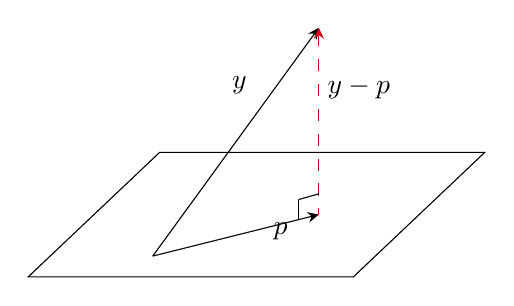
\begin{tikzpicture}[x=0.75pt,y=0.75pt,yscale=-1,xscale=1]
		%uncomment if require: \path (0,300); %set diagram left start at 0, and has height of 300
		
		%Shape: Parallelogram [id:dp4502347942292726] 
		\draw   (113.33,130) -- (270,130) -- (206.67,190) -- (50,190) -- cycle ;
		%Straight Lines [id:da3979852858777978] 
		\draw    (110,180) -- (187.09,160.73) ;
		\draw [shift={(190,160)}, rotate = 165.96] [fill={rgb, 255:red, 0; green, 0; blue, 0 }  ][line width=0.08]  [draw opacity=0] (5.36,-2.57) -- (0,0) -- (5.36,2.57) -- (3.56,0) -- cycle    ;
		%Straight Lines [id:da3930974235372434] 
		\draw    (110,180) -- (188.24,72.43) ;
		\draw [shift={(190,70)}, rotate = 126.03] [fill={rgb, 255:red, 0; green, 0; blue, 0 }  ][line width=0.08]  [draw opacity=0] (5.36,-2.57) -- (0,0) -- (5.36,2.57) -- (3.56,0) -- cycle    ;
		%Straight Lines [id:da43944712687476517] 
		\draw [color={rgb, 255:red, 208; green, 2; blue, 27 }  ,draw opacity=1 ] [dash pattern={on 4.5pt off 4.5pt}]  (190,73) -- (190,160) ;
		\draw [shift={(190,70)}, rotate = 90] [fill={rgb, 255:red, 208; green, 2; blue, 27 }  ,fill opacity=1 ][line width=0.08]  [draw opacity=0] (5.36,-2.57) -- (0,0) -- (5.36,2.57) -- (3.56,0) -- cycle    ;
		%Straight Lines [id:da4075325003962833] 
		\draw    (190,150) -- (180.2,152.8) ;
		%Straight Lines [id:da9654224371843569] 
		\draw    (180.2,152.8) -- (180.2,162.4) ;
		
		% Text Node
		\draw (167,162.4) node [anchor=north west][inner sep=0.75pt]    {$p$};
		% Text Node
		\draw (147,92.4) node [anchor=north west][inner sep=0.75pt]    {$y$};
		% Text Node
		\draw (193,92.4) node [anchor=north west][inner sep=0.75pt]    {$y-p$};
		
		
	\end{tikzpicture}
\end{figure}
	
	So we can write
	\[ \norm{y-p}^2 = \norm{y}^2 + \norm{p}^2. \]
	Using the fact that $ \norm{y}^2 = \abs{\alpha}^2 + \abs{\beta}^2 $ and $ \norm{p}^2 = \abs{\alpha}^2 + \abs{\beta}^2 $ one gets
	\[ \norm{y-p} = 0. \]
	Using the properties of the norm we have
	\[ y= p. \]
	
	To show that $ A $ is linearly independent, consider the following linear combination
	\[ \alpha x_1 + \beta x_2 = 0. \]
	By applying $ \innerProd{x_1}{\cdot} $ and $ \innerProd{x_2}{\cdot} $ to both sides one gets
	\[ \alpha =0, \qquad \beta = 0. \]
	So $ A $ is a linearly independent set of vectors. 
\end{solution}

\begin{problem}
	Let $ X $ be the linear space $ L_2[0,2\pi] $ and $ A $ the set of all functions $ x_n(t) = e^{int} $, $ n=0,1,2,\cdots $. Show that $ A $ is linearly independent.
\end{problem}
\begin{solution}
	In order not to deal with messy sums, we demonstrate the linear independence of the subset $ \set{1,e^{it},e^{2it}} $. The linear independence for arbitrary finite subset of $ A $ can be shown in a similar way. Consider
	\[ \alpha_0 + \alpha_1 e^{it} + \alpha_2e^{2it} = 0. \]
	It follows that $ \alpha_0 =0 $. Furthermore, differentiating both sides and dividing by $ ie^{it} $ one gets
	\[ \alpha_1 + 2\alpha_2 e^{2it} = 0. \]
	This time we get $ \alpha_1 = 0 $. Differentiating again and dividing by $ e^{2it} $ one gets
	$ \alpha_2 = 0 $. So $ \set{1,e^{it},e^{2it}}  $ is linearly independent.
\end{solution}

\begin{problem}
	Show that a finite set $ A = \set{x_1,\cdots,x_n} $ is a linear space $ X $ is linearly independent if and only if the only $ n $-tuple of scalars satisfying the equation
	\[ a_1x_1 + \cdots + a_nx_n = 0 \]
	is $ a_1 = \cdots = a_n = 0. $.
\end{problem}
\begin{solution}
	Assume $ A $ is linearly independent. We want to show $ a_1x_1 + \cdots + a_n x_n = 0 $ implies $ a_1=\cdots=a_n=0 $. We show this by contrapositive. Let $ a_1x_1 + \cdots + a_n x_n = 0 $ with not all of $ a_i $ equal to zero. Then one can write \[ x_i = \beta_1 x_1 + \cdots + \beta_n x_n \], where $ x_i $ is the vector that its corresponding coefficient $ \alpha_i $ was not zero. This implies that the set $ A $ is not linearly independent.
	
	For the converse we want to show $ a_1x_1 + \cdots + a_nx_n = 0 $ implying $ a_i = 0 $ for all $ i $ implies $ A $ is linearly independent. We do it by proof by contrapositive. Assume $ A $ is not linearly independent. WLOG we can assume $ x_1 $ is linear combination of others: 
	\[ x_1 = \sum_{i=2}^{n} \alpha x_i. \]
	Rearranging this sum one gets
	\[ x_1 - \alpha_2x_2 - \cdots - \alpha_nx_n = 0 \]
	with not all of coefficients equal to zero. This finishes the proof.
\end{solution}


\begin{problem}
	Let $ X $ be the linear space $ \R^n $, and let $ A $ be the set containing the $ n $ vectors
	\[ x_i = (x_{1i},x_{2i},\cdots,x_{ni}) \quad \text{for $ i=1,\cdots, n $}. \]
	Show that this set is linearly independent if and only if
	\[ \det\begin{bmatrix}
		x_{11} & x_{12} &  \cdots & x_{1n} \\
		x_{21} & x_{22} & \cdots & x_{2n} \\
		\vdots & \vdots & \ddots & \vdots \\
		x_{n1} & x_{n2} & \cdots & x_{nn}
	\end{bmatrix} \neq 0.\]
\end{problem}
\begin{solution}
	Assume the determinant is non zero and we want to show that $ A $ is linearly independent. We do this by contrapositive. Assume $ A $ is not linearly independent. So we can write one column of the matrix as the linear combination of the other column. Then by elementary column operations (that keeps the determinant intact) one can reduce that column to zero column and hence the determinant will be zero.
	
	Now assume $ A $ is linearly independent and we want to show that the determinant is non-zero. Let $ c=(c_1,\cdots,c_n) $ be a vector of coefficients. Then columns of $ A $ being linearly independent is the same as saying the following system of equations has the only zero answer
	\[ Ac = 0 \quad \text{only when} c=(0,\cdots,0). \]
	In other words, $ \ker A = \set{0} $. This implies $ A $ is invertible (because it is automatically onto), and thus $ \det(A) \neq 0. $
\end{solution}




\begin{problem}
	Let the state of a dynamical system be a point in the linear space $ X = \R^n $. Let the state at time $ k=0,1,2,\cdots $ be denoted by $ x_k $. Further, suppose that the evolution of the system is characterized by a linear transformation $ T:X\to X $. In particular, $ x_k = Tx_{k-1} $. Let $ x_0 $ be an arbitrary initial state, and consider the set
	\[ A = \set{x_0, Tx_0, T^2x_0,\cdots}. \]
	Show that there exists an integer $ p $ such that for
	\[ A_p = \set{x_0,Tx_0,\cdots,T^px_0} \]
	one has $ V(A) = V(A_p) $, that is, $ A $ and $ A_p $ span exactly the same linear spaces.
\end{problem}

\begin{solution}
	Let $ A = \set{x_1,x_2,\cdots,x_N} $ be the first linearly independent vectors that appear in $ A $. Note that $ N\leq n $, as the space $ X $ is $ n $ dimensional. Let $ p=N $. Then $ \vspan{A} = \vspan{A_p} $.
\end{solution}


\begin{problem}
	Let $ X $ be the linear space made up of all real-valued random variables defined on some probability space. Let $ A $ be a set of random variables in $ X $. Show that if a random variable $ z\in X $ is stochastically independent of each random variable in $ A $, then $ z $ is ot in $ V(A) $.
\end{problem}
\begin{solution}
	STILL THINKING ON THIS.
\end{solution}

\begin{problem}
	Let $ X $ be a linear space. A set $ K\subset X $ is said to be convex if
	\[ \lambda x + (1-\lambda)y \in K \qquad (0\leq \lambda \leq 1), \]
	whenever $ x,y\in K $. Let $ K_1 $ and $ K_2 $ be two convex sets in $ X $. 
	\begin{enumerate}[(a)]
		\item Show that $ K_1\cap K_2 $ is convex.
		\item Is $ K_1\cup K_2 $ convex?
	\end{enumerate}
\end{problem}
\begin{solution}
	\begin{enumerate}[(a)]
		\item Let $ x,y\in K_1\cap K_2 $. Then since $ K_1 $  and $ K_2 $ are convex we have
		\[ \lambda x + (1-\lambda)y \in K_1 \quad \lambda x + (1-\lambda)y \in K_2 \quad (0\leq \lambda \leq 1). \]
		Thus $ \lambda x + (1-\lambda) y \in K_1\cap K_2 $ for $ \lambda \in [0,1] $. Thus $ K_1\cap K_2 $ is convex.
		
		\item No. Let $ x_1,x_2 \in X $ be two points in the vector space. Each of the sets $ \set{x_1} $ and $ \set{x_2} $ are convex, but $ \set{x_1,x_2}$ is not.
	\end{enumerate}
\end{solution}

\begin{problem}
	Let $ y = f(x) $ be a $ C^2 $ function defined for $ -\infty < x <\infty $. Find a condition on $ d^2f/dx^2 $ in order that
	\[ K = \set{(x,y)\in \R^2: y\geq f(x)} \]
	be convex.
\end{problem}
\begin{solution}
	We use the fact that $ f''>0 $ implies $ f $ is convex, i.e. 
	\[ f(\lambda x_1 + (1-\lambda)x_2) \leq \lambda f(x_1) + (1-\lambda) f(x_2), \qquad \lambda\in [0,1] \]
	Choose $ (x_1,y_1),(x_2,y_2) \in K $. So by definition $ y_1 \geq f(x_1) $ and $ y_2 \geq f(x_2) $. Thus
	\[ f(\lambda x_1 + (1-\lambda)x_2) \leq \lambda y_1 + (1-\lambda) y_2, \qquad \lambda\in [0,1].  \]
	So $ \lambda y_1 + (1-\lambda) y_2 \in K  $ for all $ \lambda $. Thus $ K $ (the epigraph of $ f $) is convex if and only if $ f'' >0 $.
\end{solution}


\subsection{Hamel Basis}

\begin{problem}
	Prove the Rank-Nullity Theorem. I.e. for a linear map $ L: V\to W $ we have
	\[ \mathcal{R}(L) + \mathcal{N}(L) = \dim V, \]
	where
	\[ \mathcal{R}(L) = \dim\operatorname{Image}(L),\qquad \mathcal{N}(L) = \dim\ker(L) \]
\end{problem}
\begin{solution}
	Let $ B_\mathcal{N} $ be a basis for $ \mathcal{N}(L) $. We can extend this basis to a basis to the whole space:
	\[ B = B_\mathcal{R} \cup B_\mathcal{N}. \]
	So we have
	\[  \dim V = \abs{B} = \abs{B_\mathcal{R}} + \abs{B_\mathcal{N}}. \]
	We already have $ \abs{B_\mathcal{N}} = \dim \ker(L) = \mathcal{N}(L) $. Thus it remains to show $ B_\mathcal{R} = \mathcal{R}(L) = \dim\operatorname{Image}(L) $. To see this we need to show that $ L(B_\mathcal{R}) $ is linearly independent. Consider
	\[ 0 = \sum_{i=1}^{n}\alpha_i L(x_i), \qquad x_i \in B. \]
	Applying $ L $ and using linearity one gets
	\[ L(\sum_{i=1}^{n}\alpha_i x_i) = 0. \]
	However, $ x_i\notin B_\mathcal{N} $ for all $ i $. So this implies that $ \alpha_i = 0 $ for all $ i $. Hence $ L(B_\mathcal{R}) $ is linearly independent and using that fact that it spans $ \operatorname{Image}(L) $ we conclude that it is a basis for the image of $ L $, thus $ \dim\operatorname{Image}(L) = \abs{B_\mathcal{R}} $.
\end{solution}


\begin{problem}
	Let $ X $ be a finite-dimensional space with $ \dim(X) = n $. Show that every set containing $ n+1 $ points is linearly dependent.
\end{problem}
\begin{solution}
	Assume otherwise. If there are $ n+1 $ vectors linearly independent in the set, then there is a basis that contains those linearly independent vectors (or in other words, this set can be extended to a basis for the whole space). So that dimension of the space should be at least $ n+1 $, which a contradiction.
\end{solution}



\begin{problem}
	Let $ A $ be a linear subspace of a linear space $ X $. Show that $ \dim(A)\leq \dim(X) $. Moreover, if $ X $ is finite dimensional and $ A $ is a proper linear subspace of $ X $, show that $ \dim(A) < \dim(X) $.
\end{problem}
\begin{solution}
	There exists a basis for the subspace $ A $ that can further be extended to a basis for the whole space. 
	\begin{enumerate}
		\item In the case that $ X $ is finite dimensional, then it implies that the cardinality of the basis for $ X $ is at least the cardinality of $ A $, thus $ \dim A \leq \dim X $.
		\item In the case that $ X $ is infinite dimensional (countable), then if $ X $ is finite dimensional then we automatically have $ \dim A \leq \dim X $ and if $ X $ is also infinite dimensional (countable), then $ \dim A = \dim X $.
		\item In the case that $ X $ infinite dimensional (uncountable, equal to $ \mathfrak{c} $), then if $ A $ either finite or countable we will have $ \dim A \leq \dim X $ and if $ A $ is also infinite dimensional (uncountable, equal to $ \mathfrak{c} $) then we will have $ \dim A = \dim X $.
	\end{enumerate}
	
	For the case that $ X $ is finite dimensional and $ A $ is a proper subset of $ X $, let $ B_A $ be a basis for $ A $ and extend it to a basis for $ X $ called $ B_X $. Then $ B_X\backslash B_A \neq \emptyset $ (otherwise $ A $ is not a proper subspace. That is because $ \vspan{B_A} $ is the smallest subspace that contains $ A $ and if it contains all the elements that $ B_X $ has then it should be at least the whole space $ A\supseteq X $. And using $ A\subset X $ one reaches to the contradiction). This implies there are vectors in $ B_X $ that is not in $ B_A $. So $ \dim A \leq \dim X $.
\end{solution}


\begin{problem}
	Consider the following differential equation defined on $ C^2[0,\infty) $
	\[ \frac{d^2x}{dt^2} + b\frac{dx}{dt} + cx = 0. \]
	If $ X $ denotes the set of all solutions of the equation above, show that $ X $ is a linear subspace of $ C^[0,\infty) $ and that $ \dim(X) = 2 $.
\end{problem}
\begin{solution}
	Let $ X \subset C^2[0,\infty) $ be the set of all solutions to the differential equation. Observe that one can write the equation as
	\[ (\frac{d^2}{dt^2} + b\frac{d}{dt} + c)x = \mathcal{L}x = 0, \]
	where $ \mathcal{L}: C^2[0,\infty) \to C^2[0,\infty) $ is a linear operator. Then the solution set $ X $ is in fact the pre-image of the origin $ 0\in \R $, i.e. the kernel of the linear operator. The kernel of any linear operator is a linear subspace. So $ X $ is a linear subspace. One can transform this second order equation into a system of first order equations by letting:
	\[ \phi_0 = x, \qquad \phi_1 = x' \]
	Thus the equivalent equation (that its solutions are in one-to-one correspondence with the solutions of $ \mathcal{L}x=0 $) will be
	\[ \Phi' = A\Phi \]
	where $ A $ is the companion matrix of the polynomial $ t^2 + bt+c = 0 $. The ODE above has the solution
	\[ \Phi(t) = e^{At} \Phi(0). \]
	Thus every solution is characterized by $ \Phi(0) = (\phi_0(0),\phi_1(0)) = (x(0),x'(0)) $.
\end{solution}
\begin{remark}
	One can solve this problem more ``manually'', the way that Braun did in Theorem 2, Page 132. I.e. to show that $ x = \alpha_1 y_1 + \alpha_2 y_2$ is a solution (where $ y_1,y_2 \in \ker \mathcal{L} $), and also showing that any solution is of this form (by utilizing uniqueness and existence theorem). But note that one must argue that $ \ker \mathcal{L} $ contains at least two elements, which can be done by transforming the second order into two first order ODEs and arguing there exist a solution for each, and utilizing those solutions to construct two solutions, i.e. $ y_1, y_2 $
\end{remark}


\begin{problem}
	Show that if $ A $ is a set in a linear space $ X $ with $ V(A) = X $, then $ A $ contains a Hamel basis of $ X $.
\end{problem}
\begin{solution}
	Let $ B \subset A $ be a maximal linearly independent subset of $ A $ (exist by Zorn's lemma). Then $ \vspan{B} = \vspan{A} $. Because otherwise, considering the fact $ B\subset A $ thus $ \vspan{B} \subset \vspan{A} $, if there exists $ a \in \vspan{A} $ such that $ a\notin \vspan{B} $, then $ B\cup \set{a} $ is a larger linearly independent subset of $ A $, contradicting the maximality of $ B $. Since $ \vspan{B} = \vspan{A} = X $, it follows that $ B $ is a basis for $ X $.
\end{solution}


\begin{problem}
	Let $ X $ be the real linear space made up of all functions of the form $ x(t) = a\cos(\omega t+\phi) $, where $ \omega $ is fixed. Show that $ B=\set{\cos\omega t, \sin\omega t} $ is a basis for $ X $.
\end{problem}




